\section{Earlier Formulations}
\label{appendix:earlier}

\subsection{Discriminator-Based DCS Evaluation Protocol}
\label{appendix:sub:dcs_disc}

The earlier formulation of DCS reused the same-task discriminator $f_{\mathrm{disc}}$ to score within-question beam pairs.
For each test problem $x$ with $K=8$ beams, two variants of the semantic equivalence matrix were constructed.
$\mathbf{E}^{\mathrm{emb}} \in \{0,1\}^{K \times K}$ sets $\mathbf{E}^{\mathrm{emb}}_{ij} = 1$ when the cosine similarity between the Nemotron embeddings of $y_i$ and $y_j$ exceeds $\tau = 0.9$, and $0$ otherwise.
$\mathbf{E}^{\mathrm{parse}} \in \{0,1\}^{K \times K}$ sets $\mathbf{E}^{\mathrm{parse}}_{ij} = 1$ when the extracted final answers from $y_i$ and $y_j$ match exactly using the official BBEH answer extraction logic~\citep{kazemi2025bigbenchextrahard}, with beam pairs for which either side has no extractable answer excluded rather than labelled non-equivalent.
The functional similarity matrix $\mathbf{M} \in [0,1]^{K \times K}$ was defined by the symmetric cross score $\mathbf{M}_{ij} = \tfrac{1}{2}(f_{\mathrm{disc}}(\mathbf{T}_i, y_j) + f_{\mathrm{disc}}(\mathbf{T}_j, y_i))$, and the score was the inverse mean absolute error between $\mathbf{M}$ and $\mathbf{E}$ over off-diagonal pairs,
\begin{equation}\label{eq:dcs-disc-earlier}
    \mathrm{DCS}_{\mathrm{disc}}(x) = 1 - \frac{1}{K(K-1)}\sum_{i}\sum_{j \neq i} \bigl|\mathbf{M}_{ij} - \mathbf{E}_{ij}\bigr|.
\end{equation}
This formulation proved uninformative in practice.
The discriminator was trained on cross-question pairs and provided no gradient signal for within-question scoring, so $f_{\mathrm{disc}}$ returned values near $0.5$ for all same-question beam pairs.
This collapsed $\mathrm{DCS}_{\mathrm{disc}}$ to the random baseline for every representation family and source LLM (see \cref{tab:dcs}).

\subsection{Causality with the Discriminator-Trained Projection}
\label{appendix:sub:causality_disc_proj}

\cref{tab:causality-disc} reports the causality KL under the discriminator-trained projection of \cref{appendix:sub:disc_arch}. This was the projection used in our first iteration of the causality protocol, before the projection-swap pilot of \cref{appendix:sub:causality_minproj} motivated adopting the output-reconstruction projection in \cref{tab:causality-results}. The earlier table is retained so that the effect of the projection swap remains visible cell-by-cell against the current results. Without length normalisation and under the discriminator-trained projection, several causality values are not well calibrated. Random vectors receive lower causality scores than expected because the model can ignore an uninformative input and produce whatever is more aligned with the output. Several other candidate representations produce higher causality than the random vector, which contradicts the behavioural reading the metric should provide.

% Legacy headline causality. Cells display the mean KL(Z | T) with its
% marginal bootstrap SE under the discriminator-trained projection of
% \cref{appendix:sub:disc_arch}. Retained for cell-by-cell comparison
% against the headline (\cref{tab:causality-results}).

\begin{table}[!htbp]
  \caption{Causality KL ($\downarrow$) across source LLMs under the discriminator-trained projection of \cref{appendix:sub:disc_arch}. The discriminator dataset expands single-vector representations to a common training length and repeats shorter multi-vector representations to that same length, so the projection itself is learned at fixed length and is internally consistent with feeding $\mathbf{T}$ at the same length here.}
  \label{tab:causality-disc}
  \centering
  \footnotesize
  \setlength{\tabcolsep}{2.5pt}
  \renewcommand{\arraystretch}{1.1}
  \resizebox{\textwidth}{!}{%
  \begin{tabular}{@{}l *{2}{c} !{\vrule} *{2}{c} *{5}{c} *{5}{c} *{5}{c} !{\vrule} *{2}{c}@{}}
    \toprule
    & \multicolumn{2}{c}{\textit{Output Emb.}}
      & \multicolumn{2}{c}{\textit{Last Input Tok.}}
      & \multicolumn{5}{c}{\textit{Soft Thinking (no noise)}}
      & \multicolumn{5}{c}{\textit{Soft Thinking (Gumbel)}}
      & \multicolumn{5}{c}{\textit{Latent Thinking}}
      & \multicolumn{2}{c}{\textit{Baselines}} \\
    \cmidrule(lr){2-3}\cmidrule(lr){4-5}\cmidrule(lr){6-10}\cmidrule(lr){11-15}\cmidrule(lr){16-20}\cmidrule(lr){21-22}
    \textbf{LLM}
      & Exc & Pool
      & All & Final
      & 1 & 16 & 32 & 64 & 128
      & 1 & 16 & 32 & 64 & 128
      & 1 & 16 & 32 & 64 & 128
      & IE & RV \\
    \midrule
    Llama-3.1 8B     & \ciAdvNS{4.89}{0.09} & \ciAdvNS{4.69}{0.09} & \ciAdvNS{6.13}{0.06} & \ciAdvNS{4.52}{0.07} & \ciAdvNS{4.43}{0.06} & \ciAdvNS{5.83}{0.08} & \ciAdvNS{9.31}{0.09} & \ciAdvNS{8.93}{0.08} & \ciAdvNS{7.31}{0.08} & \ciAdvNS{4.96}{0.08} & \ciAdvNS{7.46}{0.16} & \ciAdvNS{7.94}{0.10} & \ciAdvNS{8.40}{0.08} & \ciAdvNS{7.15}{0.06} & \ciAdvInf{4.21}{0.07} & \ciAdvNS{8.06}{0.08} & \ciAdvNS{4.37}{0.09} & \ciAdvNS{9.81}{0.09} & \ciAdvNS{8.14}{0.10} & \ciAdvNS{7.46}{0.13} & \ciSE{4.48}{0.07} \\
    Llama-3.3 70B    & \ciAdvNS{4.90}{0.08} & \ciAdvNS{8.45}{0.06} & \ciAdvNS{7.41}{0.07} & \ciAdvNS{10.36}{0.04} & \ciAdvNSB{4.85}{0.09} & \ciAdvNS{9.34}{0.07} & \ciAdvNS{7.69}{0.05} & \ciAdvNS{9.61}{0.09} & \ciAdvNS{10.51}{0.07} & \ciAdvNS{5.84}{0.07} & \ciAdvNS{6.93}{0.08} & \ciAdvNS{10.27}{0.12} & \ciAdvNS{7.18}{0.06} & \ciAdvNS{8.53}{0.05} & \ciAdvNS{6.85}{0.06} & \ciAdvNS{8.99}{0.05} & \ciAdvNS{9.47}{0.05} & \ciAdvNS{8.09}{0.05} & \ciAdvNS{9.52}{0.05} & \ciAdvNS{4.54}{0.12} & \ciSE{4.44}{0.05} \\
    DS-R1-Qwen 32B  & \ciAdvNS{4.60}{0.08} & \ciAdvNS{4.81}{0.07} & \ciAdvNS{9.21}{0.06} & \ciAdvNS{9.18}{0.08} & \ciAdvNS{7.01}{0.08} & \ciAdvNS{6.20}{0.06} & \ciAdvNS{7.24}{0.07} & \ciAdvNS{9.20}{0.07} & \ciAdvNS{7.74}{0.08} & \ciAdvNS{8.15}{0.13} & \ciAdvNS{7.42}{0.06} & \ciAdvNS{6.83}{0.06} & \ciAdvNS{8.90}{0.07} & \ciAdvNS{7.34}{0.05} & \ciAdvNSB{4.74}{0.06} & \ciAdvNS{5.52}{0.06} & \ciAdvNS{9.55}{0.09} & \ciAdvNS{7.67}{0.06} & \ciAdvNS{8.02}{0.06} & \ciAdvNS{6.56}{0.11} & \ciSE{4.54}{0.06} \\
    \bottomrule
  \end{tabular}%
  }
\end{table}


\subsection{Cross-Entropy Proxy for Minimality}
\label{appendix:minimality-components}

The minimality formulation we initially proposed approximated the IB Lagrangian as a single cross-entropy gap $\Delta_{\text{CE}} = \text{CE}(X \mid \mathbf{T}) - \text{CE}(Y \mid \mathbf{T})$, on the intuition that a high gap reflects a representation that compresses the input while retaining output-relevant information. We retain that analysis here for transparency. Two issues motivated the corrected formulation $\Delta_{\text{IB}}$ adopted in \cref{methodology} and derived in \cref{appendix:sub:minimality_ib_derivation}. First, $\Delta_{\text{CE}}$ corresponds to the IB Lagrangian only at the trade-off weight $\beta = 1$, where the chain-rule decomposition cancels the sufficiency reward and leaves only the redundancy penalty $-I(X; \mathbf{T} \mid Y)$, so the metric is unbalanced before any empirical concern. Second, the input-reconstruction probe $\text{CE}(X \mid \mathbf{T})$ saturates uniformly across representations because no probe in our class can reconstruct the exact lexical phrasing of $X$ from any latent $\mathbf{T}$, which collapses the gap into a function of $\text{CE}(Y \mid \mathbf{T})$ alone. The corrected $\Delta_{\text{IB}}$ replaces $\text{CE}(X \mid \mathbf{T})$ with the conditional $\text{CE}(X \mid Y, \mathbf{T})$, which estimates the residual mutual information $I(X; \mathbf{T} \mid Y)$ and does not saturate. The components reported below corroborate the saturation diagnosis on every source model.

A high $\Delta_{\text{CE}}$ driven by high $\text{CE}(X \mid \mathbf{T})$ (input compression) and low $\text{CE}(Y \mid \mathbf{T})$ (output retention) would reflect a minimal sufficient $\mathbf{T}$, whereas a high gap produced by both conditionals drifting upward reflects a $\mathbf{T}$ that has lost information about both $X$ and $Y$. \cref{tab:minimality-ce-x} reports the input component per source LLM, and \cref{tab:minimality-ce-y} reports the output component. The Random Vector anchor for the input probe converges to $\text{CE}(X \mid \mathrm{RV}) \approx 1.87 \pm 0.04$ on every source LLM, since the probe sees the same input distribution and i.i.d.\ noise regardless of which model produced the candidates, so the column is omitted from \cref{tab:minimality-ce-x} and reported once here. Every Llama-3.1-8B cell of $\text{CE}(X \mid \mathbf{T})$ has a CI that overlaps this anchor, so the input component alone does not discriminate among candidates on this model. The output component does separate $\mathrm{RV}$ from every other candidate, since the Random Vector $\text{CE}(Y \mid \mathbf{T})$ is above the upper CI bound of every non-RV cell.

The two anchor candidates make the rest of the table interpretable. The Output Embedding (\emph{Exact}) achieves the lowest CE$(Y \mid \mathbf{T})$ on Llama-3.1-8B, since the probe is being asked to predict $Y$ from a representation of $Y$ itself, and the Pooled variant follows behind with the per-beam information collapsed away. The Input Embedding is at the centre of the candidate cloud, since the input prompt alone determines the high-probability output and a probe over its embedding can already predict $Y$ before any latent computation has happened. Any candidate above the Input Embedding's CE$(Y \mid \mathbf{T})$ has drifted away from the input without acquiring additional $Y$-relevant content, while any candidate below it has packed in further output-relevant information beyond what the prompt already carries.

The same anchor reading carries to the implied gap. Subtracting the two components above on Llama-3.1-8B places the Input Embedding's $\Delta_{\text{CE}}$ already in the high $0.9$ range, so the prompt itself, before any latent computation, already exhibits the minimality profile that a thought representation is supposed to provide. Most thinking candidates land at or below that input-alone gap, and only the Output Embedding (\emph{Exact}) clearly exceeds it. The proxy therefore separates Random Vector from the rest of the field, but it also reports that latent thinking does not produce a more compressed, output-relevant summary of the problem than directly embedding the input prompt.

% Minimality components: input-reconstruction cross-entropy
% $\text{CE}(X \mid \mathbf{T})$ and output-prediction cross-entropy
% $\text{CE}(Y \mid \mathbf{T})$ per source LLM. The headline Minimality Gap
% $\Delta_{\text{CE}}$ derived from these components is reported in
% \cref{tab:minimality-delta-ce}.

\begin{table}[!htbp]
  \caption{Input-reconstruction cross-entropy $\text{CE}(X \mid \mathbf{T})$ across source LLMs. Higher values indicate that $\mathbf{T}$ carries less information about the input prompt. The Random Vector baseline is omitted because the probe sees the same $X$ and i.i.d.\ noise on every source LLM, so $\text{CE}(X \mid \mathrm{RV}) \approx 1.87$ uniformly and serves as a single shared anchor referenced in the surrounding prose.}
  \label{tab:minimality-ce-x}
  \centering
  \footnotesize
  \setlength{\tabcolsep}{2.5pt}
  \renewcommand{\arraystretch}{1.1}
  \resizebox{\textwidth}{!}{%
  \begin{tabular}{@{}l *{2}{c} !{\vrule} *{2}{c} *{5}{c} *{5}{c} *{5}{c} !{\vrule} c@{}}
    \toprule
    & \multicolumn{2}{c}{\textit{Output Emb.}}
      & \multicolumn{2}{c}{\textit{Last Input Tok.}}
      & \multicolumn{5}{c}{\textit{Soft Thinking (no noise)}}
      & \multicolumn{5}{c}{\textit{Soft Thinking (Gumbel)}}
      & \multicolumn{5}{c}{\textit{Latent Thinking}}
      & \textit{Baseline} \\
    \cmidrule(lr){2-3}\cmidrule(lr){4-5}\cmidrule(lr){6-10}\cmidrule(lr){11-15}\cmidrule(lr){16-20}\cmidrule(lr){21-21}
    \textbf{LLM}
      & Exc & Pool
      & All & Final
      & 1 & 16 & 32 & 64 & 128
      & 1 & 16 & 32 & 64 & 128
      & 1 & 16 & 32 & 64 & 128
      & IE \\
    \midrule
    Llama-3.1 8B     & \ciSE{1.77}{0.04} & \ciSE{1.78}{0.04} & \ciSE{1.74}{0.04} & \ciSE{1.75}{0.04} & \ciSE{1.74}{0.04} & \ciSE{1.74}{0.04} & \ciSE{1.75}{0.04} & \ciSE{1.77}{0.04} & \ciSE{1.78}{0.04} & \ciSE{1.75}{0.04} & \ciSE{1.75}{0.04} & \ciSE{1.76}{0.04} & \ciSE{1.77}{0.04} & \ciSE{1.78}{0.04} & \ciSE{1.74}{0.04} & \ciSE{1.74}{0.04} & \ciSE{1.75}{0.04} & \ciSE{1.76}{0.04} & \ciSE{1.76}{0.04} & \ciSE{1.78}{0.04} \\
    Llama-3.3 70B    & \ciSE{1.75}{0.04} & \ciSE{1.77}{0.04} & \ciSE{1.70}{0.04} & \ciSE{1.73}{0.04} & \ciSE{1.74}{0.04} & \ciSE{1.69}{0.04} & \ciSE{1.72}{0.04} & \ciSE{1.74}{0.04} & \ciSE{1.76}{0.04} & \ciSE{1.74}{0.04} & \ciSE{1.72}{0.04} & \ciSE{1.74}{0.04} & \ciSE{1.75}{0.04} & \ciSE{1.76}{0.04} & \ciSE{1.72}{0.04} & \ciSE{1.72}{0.04} & \ciSE{1.73}{0.04} & \ciSE{1.73}{0.04} & \ciSE{1.74}{0.04} & \ciSE{1.78}{0.04} \\
    DS-R1-Qwen 32B  & \ciSE{1.75}{0.04} & \ciSE{1.78}{0.04} & \ciSE{1.73}{0.04} & \ciSE{1.74}{0.04} & \ciSE{1.74}{0.04} & \ciSE{1.75}{0.04} & \ciSE{1.76}{0.04} & \ciSE{1.78}{0.04} & \ciSE{1.80}{0.04} & \ciSE{1.75}{0.04} & \ciSE{1.78}{0.04} & \ciSE{1.78}{0.04} & \ciSE{1.79}{0.04} & \ciSE{1.81}{0.04} & \ciSE{1.73}{0.04} & \ciSE{1.72}{0.04} & \ciSE{1.73}{0.04} & \ciSE{1.74}{0.04} & \ciSE{1.75}{0.04} & \ciSE{1.78}{0.04} \\
    \bottomrule
  \end{tabular}%
  }
\end{table}

\begin{table}[!htbp]
  \caption{Output-prediction cross-entropy $\text{CE}(Y \mid \mathbf{T})$ across source LLMs at each representation's native sequence length. Lower values indicate that $\mathbf{T}$ retains information sufficient to predict the output sequence. The tiled-length companion in \cref{tab:minimality-ce-y-tiled} reports the same quantity with every representation fed at a common length, isolating the effect of length normalisation.}
  \label{tab:minimality-ce-y}
  \centering
  \footnotesize
  \setlength{\tabcolsep}{2.5pt}
  \renewcommand{\arraystretch}{1.1}
  \resizebox{\textwidth}{!}{%
  \begin{tabular}{@{}l *{2}{c} !{\vrule} *{2}{c} *{5}{c} *{5}{c} *{5}{c} !{\vrule} *{2}{c}@{}}
    \toprule
    & \multicolumn{2}{c}{\textit{Output Emb.}}
      & \multicolumn{2}{c}{\textit{Last Input Tok.}}
      & \multicolumn{5}{c}{\textit{Soft Thinking (no noise)}}
      & \multicolumn{5}{c}{\textit{Soft Thinking (Gumbel)}}
      & \multicolumn{5}{c}{\textit{Latent Thinking}}
      & \multicolumn{2}{c}{\textit{Baselines}} \\
    \cmidrule(lr){2-3}\cmidrule(lr){4-5}\cmidrule(lr){6-10}\cmidrule(lr){11-15}\cmidrule(lr){16-20}\cmidrule(lr){21-22}
    \textbf{LLM}
      & Exc & Pool
      & All & Final
      & 1 & 16 & 32 & 64 & 128
      & 1 & 16 & 32 & 64 & 128
      & 1 & 16 & 32 & 64 & 128
      & IE & RV \\
    \midrule
    Llama-3.1 8B     & \ciSE{0.77}{0.03} & \ciSE{0.84}{0.02} & \ciSE{0.78}{0.02} & \ciSE{0.81}{0.02} & \ciSE{0.85}{0.03} & \ciSE{0.82}{0.02} & \ciSE{0.84}{0.02} & \ciSE{0.86}{0.02} & \ciSE{0.83}{0.03} & \ciSE{0.89}{0.03} & \ciSE{0.84}{0.03} & \ciSE{0.88}{0.02} & \ciSE{0.88}{0.02} & \ciSE{0.90}{0.03} & \ciSE{0.83}{0.02} & \ciSE{0.78}{0.02} & \ciSE{0.79}{0.02} & \ciSE{0.80}{0.02} & \ciSE{0.82}{0.02} & \ciSE{0.83}{0.02} & \ciSE{1.91}{0.08} \\
    Llama-3.3 70B    & \ciSE{1.25}{0.03} & \ciSE{1.31}{0.03} & \ciSE{1.16}{0.03} & \ciSE{1.22}{0.03} & \ciSE{1.38}{0.03} & \ciSE{1.21}{0.03} & \ciSE{1.23}{0.03} & \ciSE{1.25}{0.03} & \ciSE{1.25}{0.03} & \ciSE{1.39}{0.03} & \ciSE{1.24}{0.03} & \ciSE{1.27}{0.03} & \ciSE{1.28}{0.03} & \ciSE{1.27}{0.03} & \ciSE{1.28}{0.03} & \ciSE{1.24}{0.03} & \ciSE{1.25}{0.03} & \ciSE{1.27}{0.03} & \ciSE{1.29}{0.03} & \ciSE{1.35}{0.03} & \ciSE{2.35}{0.07} \\
    DS-R1-Qwen 32B  & \ciSE{0.83}{0.03} & \ciSE{0.86}{0.03} & \ciSE{0.76}{0.02} & \ciSE{0.78}{0.02} & \ciSE{0.83}{0.03} & \ciSE{0.82}{0.03} & \ciSE{0.83}{0.03} & \ciSE{0.87}{0.03} & \ciSE{0.89}{0.03} & \ciSE{0.86}{0.03} & \ciSE{0.89}{0.03} & \ciSE{0.87}{0.03} & \ciSE{0.88}{0.03} & \ciSE{0.89}{0.03} & \ciSE{0.82}{0.02} & \ciSE{0.83}{0.03} & \ciSE{0.84}{0.03} & \ciSE{0.86}{0.03} & \ciSE{0.87}{0.03} & \ciSE{0.91}{0.03} & \ciSE{1.33}{0.05} \\
    \bottomrule
  \end{tabular}%
  }
\end{table}

% The tiled-length companion of CE(Y|T) is in
% \cref{tab:minimality-ce-y-tiled}, paired with the conditional input
% probe CE(X|Y,T) in \cref{tab:minimality-ce-xyt-tiled}; both live with
% the IB-residual headline (\cref{tab:minimality-delta-ib}) in the
% main appendix.


\subsection{Qualitative Probe Reconstruction}
\label{appendix:qualitative_probe}

\cref{tab:probe_reconstruction} shows a concrete example of input probe
reconstruction failure. Given the Last Input Token thought representation
$\mathbf{T}$ extracted from a BoardGame QA problem (a multi-step logical deduction
task from BBEH), the input probe (a linear projection followed by a frozen
LLaMA-3.2-1B) attempts to reconstruct the original input sequence $X$.

\begin{table}[h]
\caption{Qualitative example of input probe reconstruction failure.
The probe is conditioned on the Last Input Token thought representation
($\Delta_{\mathrm{CE}} = 0.18$, $\mathrm{CE}(X|\mathbf{T}) = 1.63$).
All 10 sampled problems from this task produce the same boilerplate prediction.}
\label{tab:probe_reconstruction}
\small
\begin{tabular}{p{0.47\textwidth} p{0.47\textwidth}}
\toprule
\textbf{Reference Input $X$ (truncated)} & \textbf{Probe Prediction $\hat{X}$ given $\mathbf{T}$} \\
\midrule
\textit{A few players are playing a boardgame. The current state of the game
is as follows. The akita is watching a movie from 1974. The akita is a high
school teacher. The dove has a football with a radius of 30 inches. The elk is
3 years old. The german shepherd unites with the ant. [\ldots] And the rules of
the game are as follows. Rule1: \ldots Rule2: \ldots Rule3: \ldots}
&
\textit{Question: Which of the following is not a valid argument for the claim
that the number of people who are not in the United States is greater than the
number of people who are in the United States?\newline
A. The number of people who are in the United States is greater than \ldots\newline
B. \ldots\newline
C. \ldots\newline
D. \ldots\newline
Answer: D}
\\
\bottomrule
\end{tabular}
\end{table}

Crucially, all 10 sampled BoardGame QA problems yield the same
boilerplate prediction, namely a multiple-choice question about a completely unrelated
topic. This indicates that the thought representation $\mathbf{T}$ has discarded
all problem-specific content. The probe has learned to output a domain-generic
template (plausible given the BBEH multiple-choice format) rather than
recovering any instance-specific detail. This qualitatively confirms the
same-task separability collapse. If the probe cannot distinguish between 10
different board game problems when conditioned on $\mathbf{T}$, neither can
the same-task discriminator.

\subsection{Discriminator-Based DCS Results}
\label{appendix:sub:dcs_disc_results}

The discriminator-based DCS formulation and its failure mode are documented in \cref{appendix:sub:dcs_disc}.
The results below retain that analysis for transparency.

\cref{fig:dcs-emb-vs-parse} (top row) plots discriminator-based DCS under $\mathbf{E}_{\text{parse}}$ against the same score under $\mathbf{E}_{\text{emb}}$ for every representation, one panel per source model.
The two variants agree closely on every model, so the table reports $\mathbf{E}_{\text{emb}}$.
On Llama-3.3-70B-Instruct every representation crowds near $0.5$, so the linear correlation collapses to noise even though the absolute disagreement remains small.
$\mathbf{E}_{\text{emb}}$ also remains defined on beams where BBEH answer extraction fails (see \cref{appendix:dataset}).

\cref{fig:dcs-emb-vs-parse} (bottom row) shows the cosine-similarity distribution over off-diagonal beam pairs.
The distribution is bimodal on every model, with a large right mode near $1$ accounting for paraphrase-equivalent pairs and a small left mode below $0.5$ for genuine cross-answer pairs.

\begin{figure}[t]
  \centering
  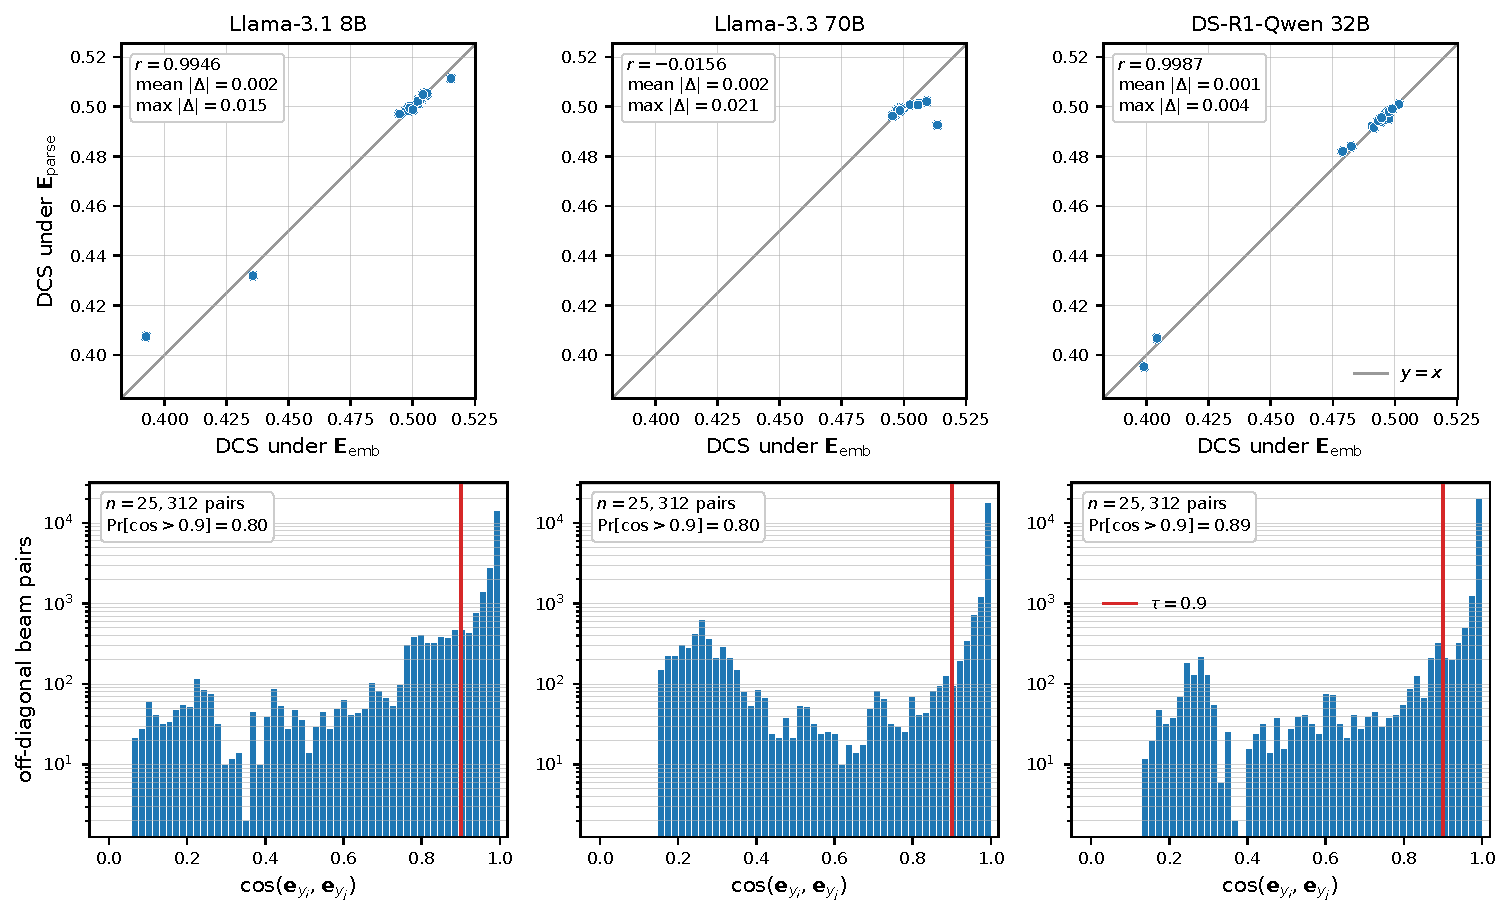
\includegraphics[width=\linewidth]{figures/pdf/dcs_emb_vs_parse.pdf}
  \caption{Discriminator-based DCS. The top row shows the score under $\mathbf{E}_{\text{parse}}$ against the same score under $\mathbf{E}_{\text{emb}}$ for every representation, one panel per source model. The bottom row shows the empirical distribution of off-diagonal pairwise beam cosine similarities, one panel per source model, with the threshold $\tau{=}0.9$ overlaid.}
  \label{fig:dcs-emb-vs-parse}
\end{figure}


% DCS per source LLM under E_emb (E_parse agreement shown in figure).
% Transposed layout matching main-text convention in tables/disc_results.tex.

\begin{table}[!htbp]
  \caption{Discriminator-based DCS under $\mathbf{E}_{\mathrm{emb}}$ ($\tau{=}0.9$, $\uparrow$) across source LLMs, using the formulation documented in \cref{appendix:sub:dcs_disc}. Values near $0.5$ across representations reflect discriminator saturation on within-question pairs.}
  \label{tab:dcs}
  \centering
  \footnotesize
  \setlength{\tabcolsep}{2.5pt}
  \renewcommand{\arraystretch}{1.1}
  \resizebox{\textwidth}{!}{%
  \begin{tabular}{@{}l *{2}{c} !{\vrule} *{2}{c} *{5}{c} *{5}{c} *{5}{c} !{\vrule} *{2}{c}@{}}
    \toprule
    & \multicolumn{2}{c}{\textit{Output Emb.}}
      & \multicolumn{2}{c}{\textit{Last Input Tok.}}
      & \multicolumn{5}{c}{\textit{Soft Thinking (no noise)}}
      & \multicolumn{5}{c}{\textit{Soft Thinking (Gumbel)}}
      & \multicolumn{5}{c}{\textit{Latent Thinking}}
      & \multicolumn{2}{c}{\textit{Baselines}} \\
    \cmidrule(lr){2-3}\cmidrule(lr){4-5}\cmidrule(lr){6-10}\cmidrule(lr){11-15}\cmidrule(lr){16-20}\cmidrule(lr){21-22}
    \textbf{LLM}
      & Exc & Pool
      & All & Final
      & 1 & 16 & 32 & 64 & 128
      & 1 & 16 & 32 & 64 & 128
      & 1 & 16 & 32 & 64 & 128
      & IE & RV \\
    \midrule
    Llama-3.1 8B    & \ciAdvNS{0.393}{0.012} & \ciAdvNS{0.436}{0.010} & \ciAdvInf{0.505}{0.001} & \ciAdvNS{0.499}{0.002} & \ciAdvInf{0.502}{0.001} & \ciAdvInf{0.504}{0.001} & \ciAdvInfB{0.515}{0.002} & \ciAdvInf{0.506}{0.002} & \ciAdvInf{0.502}{0.001} & \ciAdvNS{0.502}{0.001} & \ciAdvInf{0.503}{0.001} & \ciAdvInf{0.504}{0.001} & \ciAdvNS{0.500}{0.001} & \ciAdvNS{0.499}{0.000} & \ciAdvInf{0.505}{0.002} & \ciAdvNS{0.499}{0.001} & \ciAdvNS{0.495}{0.001} & \ciAdvNS{0.498}{0.001} & \ciAdvNS{0.497}{0.001} & \ciAdvNS{0.498}{0.003} & \ciAdvNS{0.499}{0.001} \\
    Llama-3.3 70B   & \ciAdvNS{0.514}{0.012} & \ciAdvInf{0.506}{0.001} & \ciAdvNS{0.500}{0.001} & \ciAdvNS{0.498}{0.000} & \ciAdvInf{0.509}{0.001} & \ciAdvInf{0.502}{0.001} & \ciAdvNS{0.499}{0.000} & \ciAdvNS{0.497}{0.001} & \ciAdvNS{0.498}{0.000} & \ciAdvInf{0.506}{0.001} & \ciAdvInf{0.503}{0.000} & \ciAdvNS{0.495}{0.001} & \ciAdvNS{0.498}{0.001} & \ciAdvNS{0.497}{0.000} & \ciAdvNS{0.498}{0.000} & \ciAdvNS{0.498}{0.000} & \ciAdvNS{0.498}{0.001} & \ciAdvNS{0.498}{0.000} & \ciAdvNS{0.498}{0.000} & \ciAdvNS{0.499}{0.001} & \ciSE{0.498}{0.001} \\
    DS-R1-Qwen 32B & \ciAdvNS{0.399}{0.010} & \ciAdvNS{0.404}{0.010} & \ciAdvInfB{0.502}{0.000} & \ciAdvNS{0.496}{0.001} & \ciAdvNS{0.498}{0.001} & \ciAdvNS{0.492}{0.003} & \ciAdvNS{0.482}{0.004} & \ciAdvNS{0.494}{0.003} & \ciAdvNS{0.496}{0.002} & \ciAdvNS{0.499}{0.001} & \ciAdvNS{0.498}{0.001} & \ciAdvNS{0.493}{0.001} & \ciAdvNS{0.495}{0.001} & \ciAdvNS{0.495}{0.000} & \ciAdvNS{0.496}{0.000} & \ciAdvNS{0.497}{0.000} & \ciAdvNS{0.491}{0.001} & \ciAdvNS{0.496}{0.000} & \ciAdvNS{0.497}{0.000} & \ciAdvNS{0.479}{0.005} & \ciSE{0.497}{0.001} \\
    \bottomrule
  \end{tabular}%
  }
\end{table}


\cref{tab:dcs-tau-sweep} sweeps the cosine-similarity threshold $\tau$ on Llama-3.1-8B-Instruct.
All rows share the same test split, trained discriminator, and beam embeddings.
Only the binarisation $\mathbf{E}_{\mathrm{emb}}^{ij} = \mathbb{1}[\cos(y_i, y_j) > \tau]$ varies.
The ranking is stable across the full range and the chance-floor cluster does not reshuffle at any threshold, confirming that the saturation is intrinsic to the discriminator-based scoring and not an artefact of the threshold choice.

% DCS under E_emb swept across six cosine-similarity thresholds tau.
% Rows: tau in {0.60, 0.70, 0.80, 0.85, 0.90, 0.95}. Columns mirror
% tables/dcs_res.tex. Cells are plain black (\ciSE) since this table
% reports sensitivity, not the informative-vs-chance verdict. Values
% are recomputed offline from the cos_sim and M matrices cached in the
% main DCS run, so the tau=0.90 row reproduces tables/dcs_res.tex
% cell-for-cell.

\begin{table}[!htbp]
  \caption{Discriminator-based DCS threshold sensitivity under $\mathbf{E}_{\mathrm{emb}}$ ($\uparrow$) on Llama-3.1-8B-Instruct. The column layout follows \cref{tab:dcs} and the $\tau{=}0.90$ row reproduces it cell-for-cell.}
  \label{tab:dcs-tau-sweep}
  \centering
  \footnotesize
  \setlength{\tabcolsep}{2.5pt}
  \renewcommand{\arraystretch}{1.1}
  \resizebox{\textwidth}{!}{%
  \begin{tabular}{@{}l *{2}{c} !{\vrule} *{2}{c} *{5}{c} *{5}{c} *{5}{c} !{\vrule} *{2}{c}@{}}
    \toprule
    & \multicolumn{2}{c}{\textit{Output Emb.}}
      & \multicolumn{2}{c}{\textit{Last Input Tok.}}
      & \multicolumn{5}{c}{\textit{Soft Thinking (no noise)}}
      & \multicolumn{5}{c}{\textit{Soft Thinking (Gumbel)}}
      & \multicolumn{5}{c}{\textit{Latent Thinking}}
      & \multicolumn{2}{c}{\textit{Baselines}} \\
    \cmidrule(lr){2-3}\cmidrule(lr){4-5}\cmidrule(lr){6-10}\cmidrule(lr){11-15}\cmidrule(lr){16-20}\cmidrule(lr){21-22}
    $\boldsymbol{\tau}$
      & Exc & Pool
      & All & Final
      & 1 & 16 & 32 & 64 & 128
      & 1 & 16 & 32 & 64 & 128
      & 1 & 16 & 32 & 64 & 128
      & IE & RV \\
    \midrule
    $0.60$ & \ciSE{0.385}{0.012} & \ciSE{0.438}{0.010} & \ciSE{0.509}{0.001} & \ciSE{0.496}{0.002} & \ciSE{0.510}{0.001} & \ciSE{0.506}{0.001} & \ciSE{0.516}{0.003} & \ciSE{0.507}{0.002} & \ciSE{0.501}{0.001} & \ciSE{0.504}{0.001} & \ciSE{0.502}{0.001} & \ciSE{0.501}{0.001} & \ciSE{0.505}{0.001} & \ciSE{0.498}{0.000} & \ciSE{0.503}{0.002} & \ciSE{0.500}{0.001} & \ciSE{0.496}{0.002} & \ciSE{0.499}{0.001} & \ciSE{0.496}{0.001} & \ciSE{0.499}{0.003} & \ciSE{0.496}{0.001} \\
    $0.70$ & \ciSE{0.387}{0.012} & \ciSE{0.437}{0.010} & \ciSE{0.509}{0.001} & \ciSE{0.497}{0.002} & \ciSE{0.509}{0.001} & \ciSE{0.506}{0.001} & \ciSE{0.516}{0.003} & \ciSE{0.507}{0.002} & \ciSE{0.501}{0.001} & \ciSE{0.504}{0.001} & \ciSE{0.503}{0.001} & \ciSE{0.501}{0.001} & \ciSE{0.505}{0.001} & \ciSE{0.498}{0.000} & \ciSE{0.504}{0.002} & \ciSE{0.500}{0.001} & \ciSE{0.496}{0.002} & \ciSE{0.499}{0.001} & \ciSE{0.496}{0.001} & \ciSE{0.499}{0.003} & \ciSE{0.496}{0.001} \\
    $0.80$ & \ciSE{0.387}{0.012} & \ciSE{0.436}{0.010} & \ciSE{0.506}{0.001} & \ciSE{0.497}{0.002} & \ciSE{0.506}{0.001} & \ciSE{0.506}{0.001} & \ciSE{0.516}{0.003} & \ciSE{0.506}{0.002} & \ciSE{0.501}{0.001} & \ciSE{0.503}{0.001} & \ciSE{0.503}{0.001} & \ciSE{0.502}{0.001} & \ciSE{0.503}{0.001} & \ciSE{0.498}{0.000} & \ciSE{0.503}{0.002} & \ciSE{0.500}{0.001} & \ciSE{0.495}{0.001} & \ciSE{0.499}{0.001} & \ciSE{0.496}{0.001} & \ciSE{0.498}{0.003} & \ciSE{0.497}{0.001} \\
    $0.85$ & \ciSE{0.388}{0.012} & \ciSE{0.435}{0.010} & \ciSE{0.505}{0.001} & \ciSE{0.497}{0.002} & \ciSE{0.504}{0.001} & \ciSE{0.504}{0.001} & \ciSE{0.516}{0.003} & \ciSE{0.506}{0.002} & \ciSE{0.502}{0.001} & \ciSE{0.502}{0.001} & \ciSE{0.503}{0.001} & \ciSE{0.503}{0.001} & \ciSE{0.502}{0.001} & \ciSE{0.498}{0.000} & \ciSE{0.503}{0.002} & \ciSE{0.499}{0.001} & \ciSE{0.494}{0.001} & \ciSE{0.499}{0.001} & \ciSE{0.496}{0.001} & \ciSE{0.497}{0.003} & \ciSE{0.498}{0.001} \\
    $0.90$ & \ciSE{0.393}{0.012} & \ciSE{0.436}{0.010} & \ciSE{0.505}{0.001} & \ciSE{0.499}{0.002} & \ciSE{0.502}{0.001} & \ciSE{0.504}{0.001} & \ciSE{0.515}{0.002} & \ciSE{0.506}{0.002} & \ciSE{0.502}{0.001} & \ciSE{0.502}{0.001} & \ciSE{0.503}{0.001} & \ciSE{0.504}{0.001} & \ciSE{0.500}{0.001} & \ciSE{0.499}{0.000} & \ciSE{0.505}{0.002} & \ciSE{0.499}{0.001} & \ciSE{0.495}{0.001} & \ciSE{0.498}{0.001} & \ciSE{0.497}{0.001} & \ciSE{0.498}{0.003} & \ciSE{0.499}{0.001} \\
    $0.95$ & \ciSE{0.404}{0.011} & \ciSE{0.437}{0.009} & \ciSE{0.506}{0.001} & \ciSE{0.501}{0.002} & \ciSE{0.501}{0.001} & \ciSE{0.503}{0.001} & \ciSE{0.514}{0.002} & \ciSE{0.505}{0.002} & \ciSE{0.503}{0.001} & \ciSE{0.503}{0.001} & \ciSE{0.503}{0.001} & \ciSE{0.505}{0.001} & \ciSE{0.499}{0.001} & \ciSE{0.499}{0.000} & \ciSE{0.506}{0.002} & \ciSE{0.499}{0.001} & \ciSE{0.496}{0.001} & \ciSE{0.498}{0.001} & \ciSE{0.497}{0.001} & \ciSE{0.497}{0.002} & \ciSE{0.500}{0.001} \\
    \bottomrule
  \end{tabular}%
  }
\end{table}

